\subsection{Event distribution varied with time}

In this section, we analysis how many load and drop event happened for each hour.   We divide the regions into $200m\times200m$ grids, and count the load and drop events happened in every hour. As table \ref{table_event_distribution_with_time}, the analysis results show that the total volumes of load and drop events for a week are similar, close to 2.7million. And the time periods are identical for the peak and valley of the different event quantity. 
Shown as figure \ref{figure_event_varied_w_t}, the curves of event quantity varied with time of the two kinds of event are similar, too. Which is consistent  with our experiences, because the load and drop quantity should be in balance.  What’s more, the event quantity varied with time show strong regularity—when the quantity decreases or increases is relatively certain.

\begin{table}[!h]
\caption{Events quantity varied with time}\label{table_event_distribution_with_time}
\centering
\begin{tabular}{l|c|c}
 \hline
 item &drop event quantity &load event quantity \\
  \hline
  total quatity for a week& 2,679,385&2,707,290\\
  maximum of an hour&28,583 &28,130\\
  minmum of an hour&861&918\\
  time of the peak value&2011/11/04 19:00-20:00&2011/11/04 19:00-20:00\\
  time of the valley&2011/11/03 4:00-5:00&2011/11/03 4:00-5:00\\
  \hline
  \end{tabular}
\end{table}

\begin{figure}[!h]
\centering
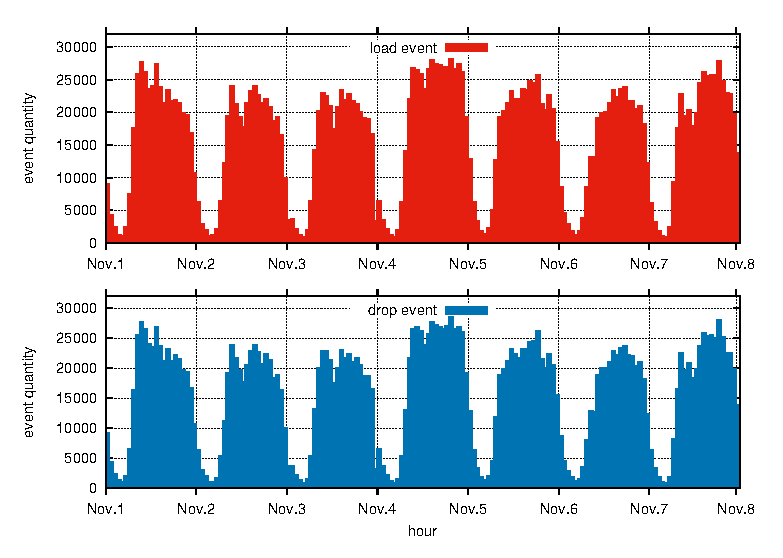
\includegraphics[width=0.5\textwidth]{figures_201103/analysis/event_w_time.eps}\\
\caption{Taxi event varied with time.}\label{figure_event_varied_w_t}
\end{figure}


From table \ref{table_event_distribution_with_time}, the peak of the event quantity happened at the same time period. In this case, we investigate the load and drop events further. By filtering the cells whose event quantities are lower than 5 per hour,  we found that although the event quantities and time periods are similar, the load and drop events tend to happen in different places. 

From 4:00 to 5:00, a hot spot of the drop events is the beijing west railway station.This may be caused by catching morning trains.
From 19:00 to 20:00, both the load and drop events happens frequently. We can figure out the main road of Beijing in figure \ref{figure_taxi_density_for_one_hour} (b) and (d). 

\begin{figure*}[!t]
\centering
\begin{tabular}
[c]{cc}
\epsfysize=2in\epsfbox{figures_201103/analysis/hotspots/hotspot_drop_04.eps} &
\epsfysize=2in\epsfbox{figures_201103/analysis/hotspots/hotspot_drop_19.eps} \\
(a) drop events at 4:00-5:00 & (b) drop events at 19:00-20:00\\
\epsfysize=2in\epsfbox{figures_201103/analysis/hotspots/hotspot_load_04.eps} &
\epsfysize=2in\epsfbox{figures_201103/analysis/hotspots/hotspot_load_19.eps} \\
(c) load events at 4:00-5:00 & (d) load events at 19:00-20:00\\
%\epsfysize=2in\epsfbox{figures_201103/analysis/hotspots/1hotspot_40_drop_19.eps} &
%\epsfysize=2in\epsfbox{figures_201103/analysis/hotspots/1hotspot_40_load_19.eps} \\
%\epsfysize=2in\epsfbox{figures_201103/analysis/hotspots/3hotspot_40_drop_19.eps} &
%\epsfysize=2in\epsfbox{figures_201103/analysis/hotspots/3hotspot_40_load_19.eps} \\
%\epsfysize=2in\epsfbox{figures_201103/analysis/hotspots/6hotspot_40_drop_19.eps} &
%\epsfysize=2in\epsfbox{figures_201103/analysis/hotspots/6hotspot_40_load_19.eps} \\
\end{tabular}
\caption{Taxi density for load/drop events in one hour.}\label{figure_taxi_density_for_one_hour}
\end{figure*}

\begin{itemize}
  \item For drop and load event, the total event number for a week are very close.
  \item The peak and valley occurs in similar time. From the data, we can find that the peak and valley happened at same time, coincidentally.
  \item The maximum event number is much larger than the minimum event number. The quantity of event number changes over time. The curves for the load and drop events follows similar rules. The quantities at the same time range are similar, too.
	\item the hotspots of the load and drop events are relatively fixed during a time peroid.
\end{itemize}

The analysis results fit with our daily experience: (1) the amount of passengers decreases early in the morning, (2) the load event quantity equilibrates with the drop event quantity, and (3) the event quantity at certain time shows certain regularity. 

